\documentclass[eikonal.tex]{subfiles}

\begin{document}

\section{Second order Eikonal OLIM}

I was a little confused about how to derive this, but I think the
thing to do is:
\begin{itemize}
\item Start with the 2nd order fast marching method Hamiltonian
\item Apply the Legendre transform
\item Consider the form of the resulting Lagrangian, and see if it's
  obvious how to derive the general Lagrangian that we would need for
  the second order OLIM
\end{itemize}

\section{High-frequency Helmholtz solver}

For a paper about the high-frequency Helmholtz solver, here are some
things that would be good to include:
\begin{itemize}
\item Algorithms for computing penumbra in 2D and 3D
\item Approaches to dealing with diffraction
\end{itemize}
And some applications:
\begin{itemize}
\item Some nice domains with complicated obstacles, e.g. the stuff for
  the multiple reflections problems
\item Measuring HRTFs of heads by emitting from ears (for
  Ramani)... This would be a great application! Since there would be
  boundaries etc.
\end{itemize}

\section{Fast olim4qpot updates}

It's not clear to me that the quasipotential OLIM solver doesn't have
complexity $O(N^{2d} + N^d \log N)$. Speeding this solver up to truly
have complexity $O(N^d \log N)$ or $O(N^d)$ would be a fun
challenge. Since a big set of update candidates has to be searched
over, it seems like it would be possible to come up with some clever
searching procedure along the lines of what we're doing before to do
this.

\section{SIMD olim4eikonal}

Is it possible to do each update phase using SIMD operations? There
are a small number of them, but, e.g., for olim4 or standard FMM, it
seems like it could be possible to just do all of the updates in
parallel and mask the ones which are valid. This might save on FLOPs.

\section{Domain decomposition}

\begin{center}
  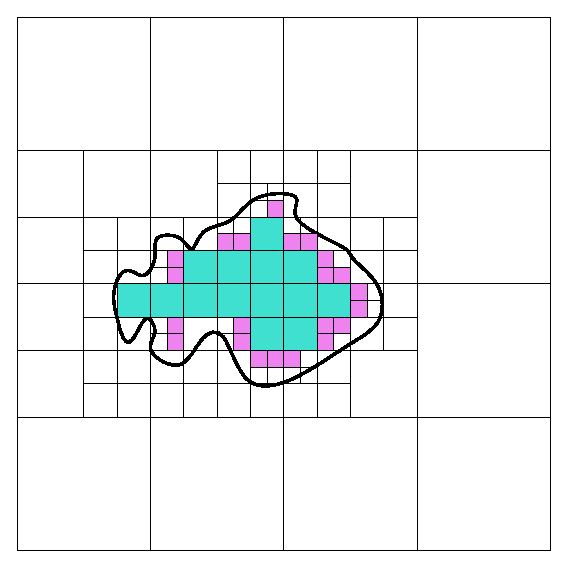
\includegraphics{domains.eps}
\end{center}

\paragraph{Questions:}
\begin{itemize}
\item Is the heap cell method relevant here?
\item Can we define an Dijkstra-like solver or sweeping method
  recursively?
\item What about ``block causality'': can we implement a Dial-like
  solver? This might actually be quite useful in this context, since
  large problems are getting to be of the size where distributing each
  problem across threads or even nodes would make sense.
\item How do we deal with hanging nodes?
\item How much can we simplify things for large blocks when the
  slowness or speed function is simple? E.g., constant slowness/speed
  or linear slowness or linear speed, where the characteristics are
  known exactly.
\end{itemize}

\section{Relationship between eikonal equation and anisotropic eikonal
  equation}

\paragraph{Eikonal $\to$ anisotropic eikonal.} Under a smooth,
nonlinear transformation that's locally invertible, an eikonal
equation that is to be solved on an unstructured grid can be
transformed into an anisotropic eikonal equation defined on a regular
grid. This could also transform an eikonal equation defined on an
unstructured grid into a structured grid, but the interpolation
problem is a little simpler in the former case.

\paragraph{Anisotropic eikonal $\to$ eikonal (lifting).} Another idea:
starting with an anisotropic eikonal equation to be solved on a grid
(say, in $\mathbb{R}^d$, $d = 2, 3$), add another dimension and solve
an eikonal equation on a $d$-dimensional surface (that's a graph of a
function) embedded in $\mathbb{R}^{d + 1}$.

\section{Exact solution for other slowness functions}

There are other slowness functions (linear slowness, linear speed,
...?) which have exact solutions for rays. We could try coming up with
ordered line integral methods which solve local ray-tracing problems
where the solutions take these forms.

\section{Solving the discrete geodesic problem}

When we globally factor the eikonal equation, it computes the exact
set distance. We could try doing this on a triangle mesh (or
tetrahedron mesh). We could try using this as a means of solving the
discrete geodesic problem. One problem here is computing the distance
for the correct term $T$. To do this, we would need to dynamically
compute the discrete geodesics starting along line segments as we
go. This might be tricky, but in any case, it's the quantity we're
after for solving the problem.

\section{Solving a sequence of nonlinear equations}

As a label-setting method proceeds, at any given point in time, there
is an expanding wavefront of \texttt{valid} nodes. Using the finite
difference formulation, for a fixed set of \texttt{valid} nodes, each
of the bordering downwind nodes satisfy the following equation, e.g.:
\begin{equation}
  \parens{U_{ij} - U_H}^2 + \parens{U_{ij} - U_V}^2 - s_{ij}^2 h^2 = 0.
\end{equation}
This can be rewritten:
\begin{equation}
  U_{ij} = \frac{U_H + U_V}{2} + \frac{1}{2} \sqrt{\parens{U_H + U_V}^2 - 2\parens{U_H^2 + U_V^2 - s_{ij}^2 h^2}}.
\end{equation}
If we let $\m{U}$ denote the vector of unknowns at the given ``time
step'', then the first equation is written in rootfinding for some
function, $F(\m{U}) = 0$. The second is written in fixed-point form;
i.e., $G(\m{U}) = \m{U}$. Newton's method can be applied to the first,
and Picard iteration can be applied to the second---see the \emph{Acta
  Numerica} review ``Numerical Methods for Nonlinear Equations'' by
C.T. Kelley.

\emph{Update}: first attempt at this using a point source and constant
slowness function and the fixed-point form worked extremely well. There
was no need for iteration at each wave-level. Let $t \geq 0$ be the
``time index'' of the ``numerical wave'' expansion, let $k \geq 0$ be
the iteration step, and let $\mathcal{I}_t^k$ be the set of indices
that ``need updating''. It seems likely that we'll have a chain like
this:
\begin{equation}
  \mathcal{I}_t^0 \supseteq \mathcal{I}_t^1 \supseteq \cdots \supseteq \emptyset.
\end{equation}
If this is the case, we can optimize the \emph{hell} out of this
algorithm.

\emph{See Steffensen's method on Wikipedia.}

We should compare this with the $O(N)$ algorithm based on Dial's
algorithm.

\section{Adaptive line integral methods (``smartmeshing'')}

The key issue with smartmeshing is how to propagate neighborhoods from
the parent mesh to the child mesh after subdividing. Here's one
plausible way of doing it:
\begin{center}
  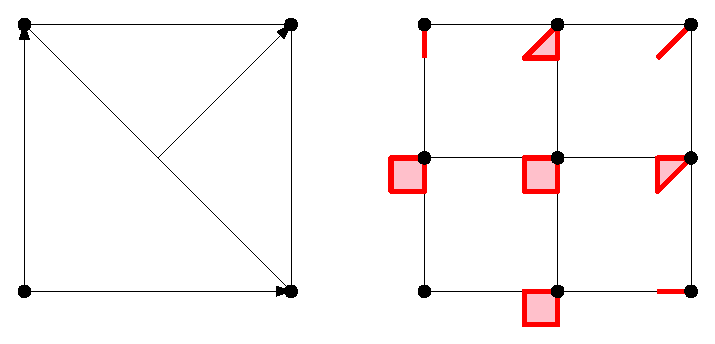
\includegraphics{recursive-neighborhoods.eps}
\end{center}
The idea is:
\begin{itemize}
\item After updating, each node will know the direction they were
  updated from---i.e. they will have a linear approximation to the
  characteristic arriving there. 
\item At intersecting nodes, we look to
  these nodes and use the convex hull of these characteristics.
\item The key issue here is the logic used to determine which nodes to
  look at. We can probably come up with something based on the order
  of the nodes' solution and the directions of the neighboring
  characteristics.
\end{itemize}

\section{Numerical study of other queueing methods}

Since my code is already very generic, it should be very easy to
extend it to use other queueing algorithms. Likewise, it should be
easy to extend it to parallel versions of these algorithms. Here are
some random HPC ideas:
\begin{itemize}
\item Dial's algorithm may not be wide enough for GPU implementation,
  but maybe it would work well using SIMD. How about using Intel ISPC
  or libsimd?
\end{itemize}

\section{Local factoring for HF acoustics}

In Qi and Vladimirsky's paper, they do local factoring by dynamically
identifying where the norm of the Hessian is singular. The Hessian
becomes singular at corners. I'm guessing this happens numerically
because they set the value of nodes that are ``part of the wall'' to
be infinity. Could an alternative approach to this be to first go
through the domain and identify sharp features of the mesh and then
just set those to be ``parent nodes''?

\section{Randomly perturbing slowness functions}

Try to characterize how much slowness functions can be randomly
perturbed by before solvers break down
\section{OLIM in $\R^n$}

\begin{itemize}
\item OLIM in higher dimensions
\item Causality will become more important
\item Need to precompute larger number of QR decompositions
\item OLIM on an adaptive mesh (approximate $k$-nearest neighbors in
  higher dimensions)
\end{itemize}

\section{Quadratic slowness function and $u$}

Higher order?

\section{Incorporate gradient of slowness function}

\begin{itemize}
\item Don't have access to analytical form: spectral differentiation
\item Do have access: take the gradient and Hessian
\end{itemize}
Either way, actually evaluate $s(\lambda)$ and use derivatives and
gradients

\section{Locally Quadratic Characteristics}
\subfile{quadratic-characteristic.tex}

\section{Optimizing $\theta$}

Let's say we incorporate $\theta$ as a parameter into our minimization
problem; i.e., we minimize:
\begin{equation}
  (\lambda^*, \theta^*) = \argmin_{\lambda \in \Delta^n, \theta \in [0, 1]} F_i(\lambda, \theta).
\end{equation}
Then, for $i = 0$, we have:
\begin{align*}
  \nabla_\lambda F_0 &= \delU + s^\theta h \delP^\top \nu_\lambda, \\
  \nabla_\lambda^2 F_0 &= \frac{s^\theta h}{l_\lambda} \delP^\top \mathcal{P}_\lambda^\perp \delP, \\
  \frac{\partial F_0}{\partial \theta} &= \delta \overline{s} h \delP^\top \nu_\lambda, \\
  \frac{\partial^2 F_0}{\partial \theta^2} &= 0, \\
  \nabla^2 F_0 &= \begin{bmatrix}
    \nabla_\lambda^2 F_0 & \frac{\partial F_0}{\partial \theta} \\
    \frac{\partial F_0}{\partial \theta}^\top & 0
  \end{bmatrix} = \begin{bmatrix}
    \frac{s^\theta h}{l_\lambda} \delP^\top \mathcal{P}_\lambda^\perp \delP & \delta \overline{s} h \delP^\top \nu_\lambda \\
    \delta \overline{s} h \nu_\lambda^\top \delP  & 0
  \end{bmatrix}.
\end{align*}
In this case, $\nabla^2 F_0$ is indefinite, so our minimization
procedure becomes more complicated. We could apply SQP again, in which
case we would need to invert $\nabla^2 F_0$. We want to take advantage
of what we've already done for $\nabla_\lambda F_0^2$. For
$A \in \mathbb{R}^{n \times n}$ and $b \in \mathbb{R}^{n}$ (playing
the roles of $\nabla_\lambda^2 F_0$ and $\partial_\theta F_0$,
respectively), we have:
\begin{align*}
  \begin{bmatrix}
    A & b \\
    b^\top &
  \end{bmatrix}^{-1} = \begin{bmatrix}
    A^{-1} - A^{-1} b (b^\top A^{-1} b)^{-1} b^\top A^{-1} & A^{-1} b (b^\top A^{-1} b)^{-1} \\
    (b^\top A^{-1} b)^{-1} b^\top A^{-1} & -(b^\top A^{-1} b)^{-1}
  \end{bmatrix}
\end{align*}
or something like it (check arithmetic). This could be simplified and
would lead to an easy SQP iteration. With this idea, we need to be
careful with the consistency of the method.

Here's some MATLAB code to play around with this:

\begin{verbatim}
h = 0.1;

p0 = [1; 0; 0]; % randn(3, 1);
p1 = [0; 1; 0]; % randn(3, 1);
dp = p1 - p0;

u = 1 + h*rand(2, 1);
s = 1 + h*rand(2, 1);
shat = 1 + h*rand();

u0 = u(1);
du = u(2) - u0;

s0 = s(1);
ds = s(2) - s0;

F0 = @(lam, th) u0 + lam*du + ((1 - th)*shat + th*(s0 + lam*ds))*h*norm(p0 + lam*dp);

[Lam, Th] = meshgrid(0:0.005:1, 0:0.005:1);

contour(Lam, Th, arrayfun(F0, Lam, Th), 30);
\end{verbatim}

\begin{center}
  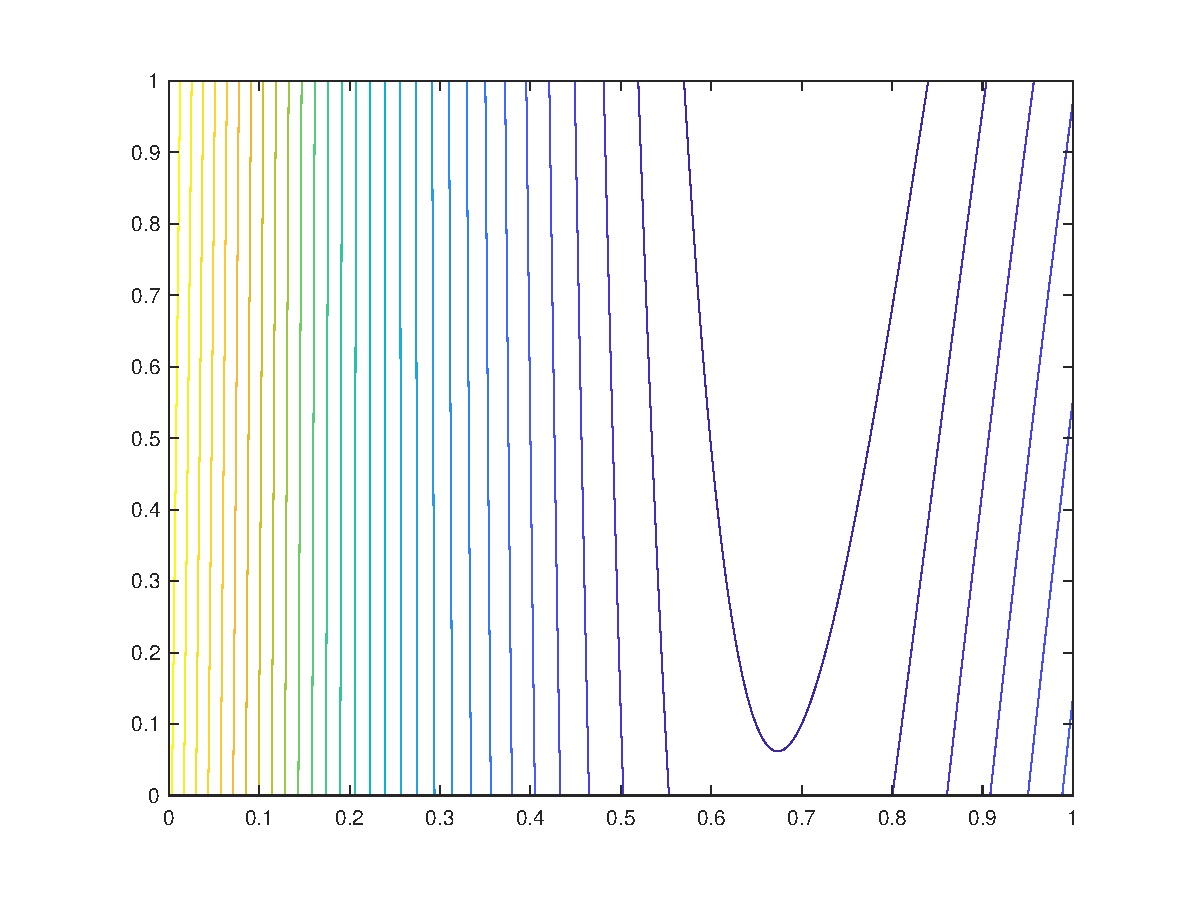
\includegraphics[width=0.6\linewidth]{saddle.eps}
\end{center}

From a plot like this, it seems like it may be possible to check
$\partial_\theta F_0$ at each point and use this value to decide
between $\theta = 0$ and $\theta = 1$.

Question: does it actually make sense to include $\theta$ as a
parameter for minimization? We're trying to find the best
approximation to the minimal line integral. Minimizing over $\theta$
will let us decrease the value but this may not actually lead to a
better approximation of the true line integral. So, this idea may not
actually make much sense...

\section{External Memory Implementation}
\begin{itemize}
\item \texttt{memmap}
\item Using different data structures for the heap and node storage:
  \begin{itemize}
  \item B-tree (for heap and/or node storage
  \item Morton order/Z-order
  \end{itemize}
\end{itemize}

\end{document}

%%% Local Variables:
%%% mode: latex
%%% TeX-master: t
%%% End:
